% Options for packages loaded elsewhere
\PassOptionsToPackage{unicode}{hyperref}
\PassOptionsToPackage{hyphens}{url}
\documentclass[
]{ltjsarticle}
\usepackage{xcolor}
\usepackage[margin=20mm]{geometry}
\usepackage{amsmath,amssymb}
\setcounter{secnumdepth}{-\maxdimen} % remove section numbering
\usepackage{iftex}
\ifPDFTeX
  \usepackage[T1]{fontenc}
  \usepackage[utf8]{inputenc}
  \usepackage{textcomp} % provide euro and other symbols
\else % if luatex or xetex
  \usepackage{unicode-math} % this also loads fontspec
  \defaultfontfeatures{Scale=MatchLowercase}
  \defaultfontfeatures[\rmfamily]{Ligatures=TeX,Scale=1}
\fi
\usepackage{lmodern}
\ifPDFTeX\else
  % xetex/luatex font selection
\fi
% Use upquote if available, for straight quotes in verbatim environments
\IfFileExists{upquote.sty}{\usepackage{upquote}}{}
\IfFileExists{microtype.sty}{% use microtype if available
  \usepackage[]{microtype}
  \UseMicrotypeSet[protrusion]{basicmath} % disable protrusion for tt fonts
}{}
\makeatletter
\@ifundefined{KOMAClassName}{% if non-KOMA class
  \IfFileExists{parskip.sty}{%
    \usepackage{parskip}
  }{% else
    \setlength{\parindent}{0pt}
    \setlength{\parskip}{6pt plus 2pt minus 1pt}}
}{% if KOMA class
  \KOMAoptions{parskip=half}}
\makeatother
\usepackage{graphicx}
\makeatletter
\newsavebox\pandoc@box
\newcommand*\pandocbounded[1]{% scales image to fit in text height/width
  \sbox\pandoc@box{#1}%
  \Gscale@div\@tempa{\textheight}{\dimexpr\ht\pandoc@box+\dp\pandoc@box\relax}%
  \Gscale@div\@tempb{\linewidth}{\wd\pandoc@box}%
  \ifdim\@tempb\p@<\@tempa\p@\let\@tempa\@tempb\fi% select the smaller of both
  \ifdim\@tempa\p@<\p@\scalebox{\@tempa}{\usebox\pandoc@box}%
  \else\usebox{\pandoc@box}%
  \fi%
}
% Set default figure placement to htbp
\def\fps@figure{htbp}
\makeatother
\setlength{\emergencystretch}{3em} % prevent overfull lines
\providecommand{\tightlist}{%
  \setlength{\itemsep}{0pt}\setlength{\parskip}{0pt}}
\usepackage{bookmark}
\IfFileExists{xurl.sty}{\usepackage{xurl}}{} % add URL line breaks if available
\urlstyle{same}
\hypersetup{
  hidelinks,
  pdfcreator={LaTeX via pandoc}}

\author{}
\date{}

\begin{document}

\section{半波長奇数倍音孤立ピーク波の二コピー共通相対位相重ね合わせにおける波形不変性とコントラスト則の観察}\label{ux534aux6ce2ux9577ux5947ux6570ux500dux97f3ux5b64ux7acbux30d4ux30fcux30afux6ce2ux306eux4e8cux30b3ux30d4ux30fcux5171ux901aux76f8ux5bfeux4f4dux76f8ux91cdux306dux5408ux308fux305bux306bux304aux3051ux308bux6ce2ux5f62ux4e0dux5909ux6027ux3068ux30b3ux30f3ux30c8ux30e9ux30b9ux30c8ux5247ux306eux89b3ux5bdf}

\textbf{副題}:
二つのコピーに共通の相対位相を与えても波形は変わらず、二乗振幅が相対位相の余弦二乗倍になる

\textbf{著者}: 木原範昭 (Noriaki Kihara)\\
\textbf{版}: v0.1\\
\textbf{日付}: 2026-06-26\\
\textbf{DOI}: Version 10.5281/zenodo.20923462（本版）/ Concept
10.5281/zenodo.20923461（外部参照用・最新版へ自動転送）\\
\textbf{Zenodo}: https://zenodo.org/records/20923462\\
\textbf{位置づけ}:
観察・整理論文としての初稿。半波長の位相区間上で一定振幅の奇数倍音を重ね合わせた孤立ピーク波について、その二つのコピーに共通の相対位相を与えて重ね合わせると、波形（形状・両端の零・局在幅）が相対位相に依存せず、二乗振幅だけが相対位相の余弦二乗に比例して変化することを、初等的なフーリエ和と三角恒等式の性質として記録する。物理法則の導出や観測事実の主張は行わず、特定の物理的解釈も与えない。

\begin{center}\rule{0.5\linewidth}{0.5pt}\end{center}

\subsection{要旨}\label{ux8981ux65e8}

半波長の位相区間 \(\varphi\in[-\pi/2,\pi/2]\)
上で、一定振幅の奇数倍音を重ね合わせた波

\[
S_N(\varphi)=\sum_{m=0}^{(N-1)/2}\cos\!\big((2m+1)\varphi\big)
\]

は中央に主ピークをもち両端で零となる孤立ピーク波である（\(N\)
は最高奇数倍音次数、\(N\) は奇数）。

本稿では、この波の二つのコピーに、全倍音へ共通の相対位相 \(2\alpha\)
を与えて重ね合わせた波

\[
\psi_\alpha(\varphi)=\sum_{m=0}^{(N-1)/2}\Big[\cos\!\big((2m+1)\varphi-\alpha\big)+\cos\!\big((2m+1)\varphi+\alpha\big)\Big]
\]

を観察する。三角恒等式から直ちに
\(\psi_\alpha(\varphi)=2\cos\alpha\cdot S_N(\varphi)\)
が成り立ち、したがって二乗振幅は
\(I_\alpha(\varphi)=4\cos^2\!\alpha\cdot S_N(\varphi)^2\)
となる。これは次の二点を意味する：(i) \textbf{波形は相対位相 \(\alpha\)
に依存しない}（規格化波形は単一コピーのものと一致する）。(ii)
\textbf{相対位相は全体の二乗振幅に余弦二乗のコントラスト因子
\(\cos^2\!\alpha\)
としてのみ現れる}。本稿はこの性質を初等的なフーリエ和と三角恒等式の観察として記録するにとどめ、物理的解釈は与えない。

\begin{center}\rule{0.5\linewidth}{0.5pt}\end{center}

\subsection{1. はじめに}\label{ux306fux3058ux3081ux306b}

一定振幅の奇数倍音のみを半波長区間上で重ね合わせると、中央に卓越した主ピークをもち両端で零となる孤立ピーク波が形成される。本稿は、この孤立ピーク波そのものの性質ではなく、その\textbf{二つのコピーを共通の相対位相のもとで重ね合わせたとき}に波形と二乗振幅がどう振る舞うかを観察する。

ここで扱う相対位相は、各倍音の位相に\textbf{共通}に加わる一定のオフセット
\(\pm\alpha\) である。すなわち、倍音次数 \(n=2m+1\)
に比例して位相がずれる量（区間内での平行移動に相当する）ではなく、全倍音に同一に課される位相量である。この区別は本稿の観察の前提であり、§2
で明示する。

記法と公式は標準的な解析学のテキスト {[}1{]}
に従う。本稿の主結果（§3）は、和積の三角恒等式
\(\cos(u-\alpha)+\cos(u+\alpha)=2\cos u\cos\alpha\)
を各倍音に適用するだけで得られる初等的な事実である。

\begin{center}\rule{0.5\linewidth}{0.5pt}\end{center}

\subsection{2. 定義}\label{ux5b9aux7fa9}

\subsubsection{2.1
孤立ピーク波}\label{ux5b64ux7acbux30d4ux30fcux30afux6ce2}

変数 \(\varphi\in[-\pi/2,\pi/2]\) で、一定振幅の奇数倍音和を

\[
S_N(\varphi)=\sum_{m=0}^{(N-1)/2}\cos\!\big((2m+1)\varphi\big)
\tag{2.1}
\]

と定義する。ここで \(N\) は最高奇数倍音次数で、\(N\) は奇数、和には
\(1,3,5,\dots,N\) の \((N+1)/2\) 個の項が含まれる。\(S_N\) は中央
\(\varphi=0\) で

\[
S_N(0)=\frac{N+1}{2}
\tag{2.2}
\]

の主ピークをもち、両端 \(\varphi=\pm\pi/2\)
で零となる。後者は、各奇数倍音が \(\cos\!\big((2m+1)(\pm\pi/2)\big)=0\)
を満たすことから、振幅 \(S_N\)
の値や項数によらず成り立つ。非負の観察量として二乗振幅

\[
I_N(\varphi)=\big|S_N(\varphi)\big|^2=S_N(\varphi)^2
\tag{2.3}
\]

を用いる。

図1に、各奇数倍音（\(n=1,3,5,7,9\)、すなわち
\(N=9\)）と、それらをコヒーレントに重ね合わせた総和（黒）を、半波長閉区間
\(\pm 90^\circ\ (=\pm\pi/2)\)
の中央領域について示す。総和が中央に主ピークをもつ孤立ピーク波となることが確認できる。

\begin{figure}
\centering
\pandocbounded{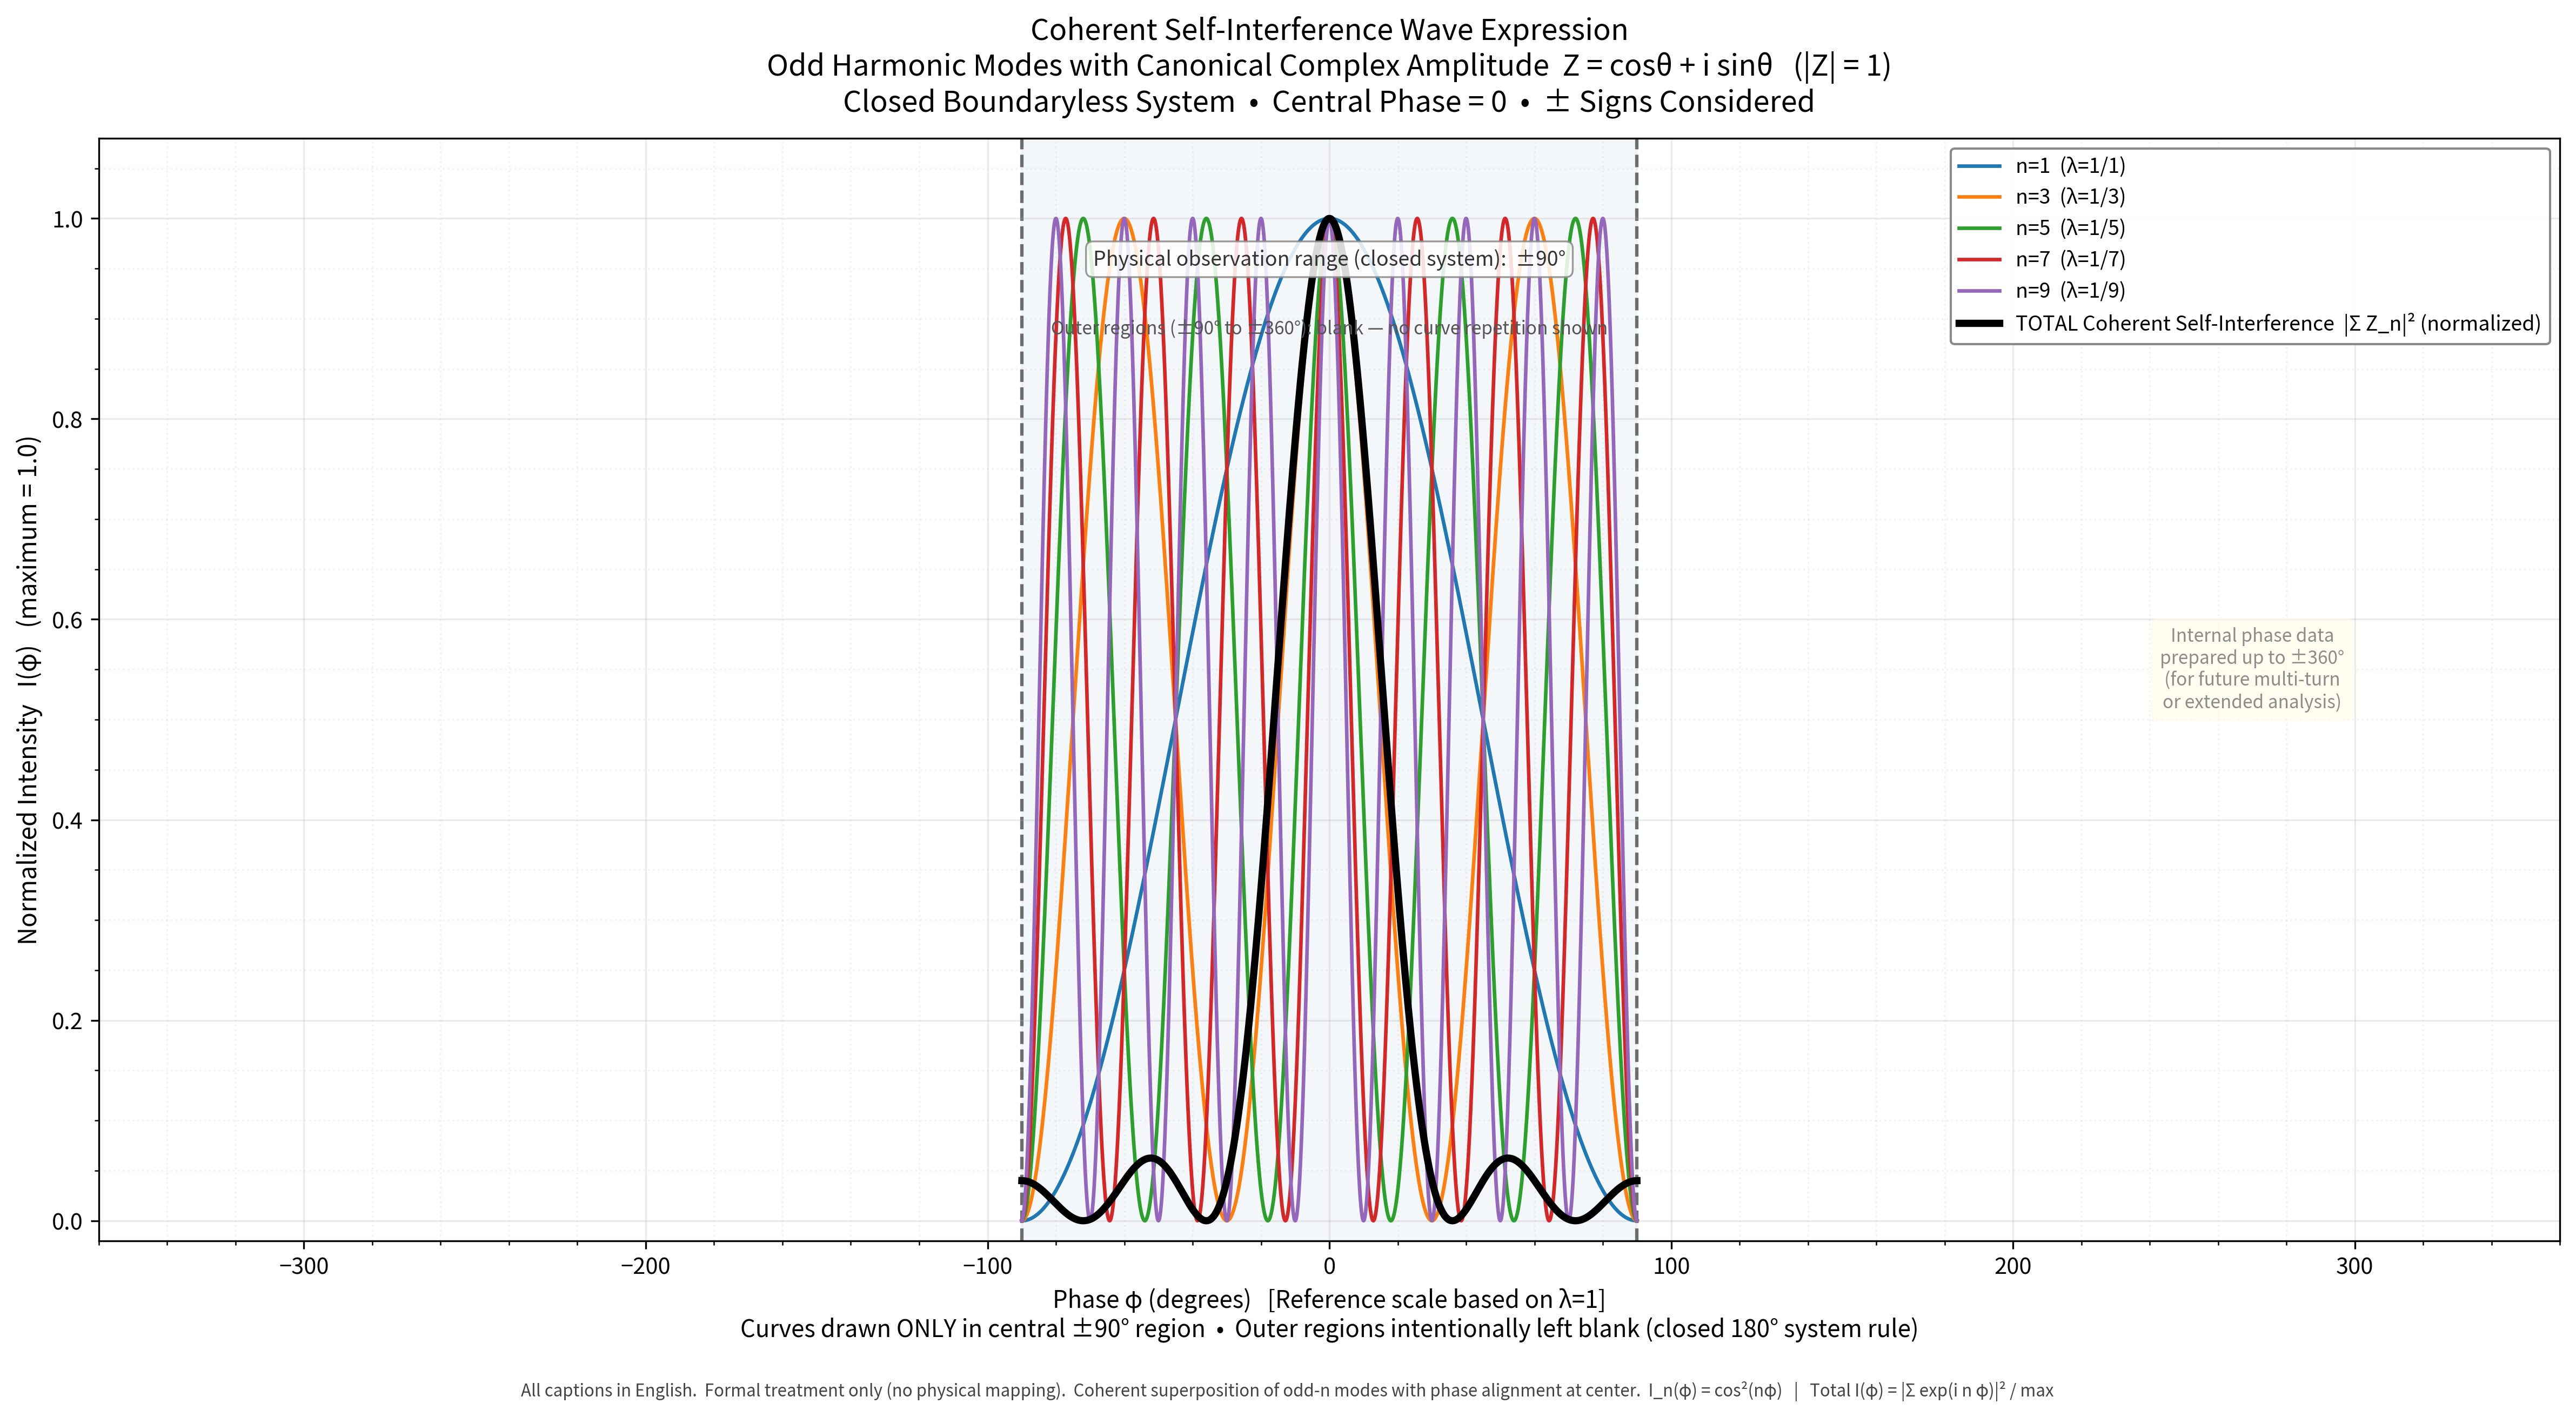
\includegraphics[keepaspectratio,alt={図1}]{coherent_self_interference_odd_modes.png}}
\caption{図1}
\end{figure}

\textbf{図1}: 一定振幅奇数倍音（\(n=1,3,5,7,9\)、正準複素振幅
\(Z=\cos\theta+i\sin\theta\)、\(|Z|=1\)）と、それらのコヒーレント和（黒）。半波長閉区間
\(\pm 90^\circ\) の中央領域に規格化して描画。

\subsubsection{2.2
共通相対位相を与えた二コピーの重ね合わせ}\label{ux5171ux901aux76f8ux5bfeux4f4dux76f8ux3092ux4e0eux3048ux305fux4e8cux30b3ux30d4ux30fcux306eux91cdux306dux5408ux308fux305b}

\(S_N\) の二つのコピーに、全倍音へ共通の相対位相 \(\pm\alpha\)
を与えて重ね合わせた波を

\[
\psi_\alpha(\varphi)
=\sum_{m=0}^{(N-1)/2}\Big[\cos\!\big((2m+1)\varphi-\alpha\big)+\cos\!\big((2m+1)\varphi+\alpha\big)\Big]
\tag{2.4}
\]

と定義する。ここで \(\alpha\) は倍音次数 \(n=2m+1\)
に依存しない一定量であり、二つのコピーの相対位相差は全倍音で一律に
\(2\alpha\) である。観察量は二乗振幅

\[
I_\alpha(\varphi)=\big|\psi_\alpha(\varphi)\big|^2=\psi_\alpha(\varphi)^2
\tag{2.5}
\]

とする。

\begin{center}\rule{0.5\linewidth}{0.5pt}\end{center}

\subsection{3.
観察：波形不変性とコントラスト則}\label{ux89b3ux5bdfux6ce2ux5f62ux4e0dux5909ux6027ux3068ux30b3ux30f3ux30c8ux30e9ux30b9ux30c8ux5247}

\subsubsection{3.1 恒等式}\label{ux6052ux7b49ux5f0f}

和積の三角恒等式

\[
\cos\!\big(n\varphi-\alpha\big)+\cos\!\big(n\varphi+\alpha\big)=2\cos\!\big(n\varphi\big)\cos\alpha
\tag{3.1}
\]

を式 (2.4) の各倍音 \(n=2m+1\) に適用すると、\(\cos\alpha\) は \(n\)
に依存しない共通因子であるから和の外に出て、

\[
\psi_\alpha(\varphi)
=2\cos\alpha\sum_{m=0}^{(N-1)/2}\cos\!\big((2m+1)\varphi\big)
=2\cos\alpha\cdot S_N(\varphi)
\tag{3.2}
\]

を得る。これは近似ではなく厳密な恒等式である。

\subsubsection{3.2
二乗振幅・不変性・コントラスト}\label{ux4e8cux4e57ux632fux5e45ux4e0dux5909ux6027ux30b3ux30f3ux30c8ux30e9ux30b9ux30c8}

式 (3.2) を二乗すると、

\[
I_\alpha(\varphi)=4\cos^2\!\alpha\cdot S_N(\varphi)^2=4\cos^2\!\alpha\cdot I_N(\varphi)
\tag{3.3}
\]

である。ここから次の二点が直ちに従う。

\textbf{(1) 波形不変性.} \(\varphi\) への依存性は
\(S_N(\varphi)^2=I_N(\varphi)\) にすべて含まれ、相対位相 \(\alpha\)
は前因子 \(4\cos^2\!\alpha\)
にのみ現れる。したがって主ピーク値で規格化した波形

\[
\widehat{I}_\alpha(\varphi):=\frac{I_\alpha(\varphi)}{I_\alpha(0)}
=\frac{4\cos^2\!\alpha\,I_N(\varphi)}{4\cos^2\!\alpha\,I_N(0)}
=\frac{I_N(\varphi)}{I_N(0)}=\widehat{I}_N(\varphi)
\tag{3.4}
\]

は \(\alpha\) に依存せず、単一コピーの規格化波形 \(\widehat{I}_N\)
と完全に一致する（\(\cos\alpha\neq0\) のとき）。形状、両端
\(\varphi=\pm\pi/2\)
の零、主ピーク近傍の局在幅は、いずれも相対位相を変えても不変である。

\textbf{(2) コントラスト則.} 規格化前のピーク二乗振幅は

\[
I_\alpha(0)=4\cos^2\!\alpha\cdot I_N(0)=(N+1)^2\cos^2\!\alpha
\tag{3.5}
\]

であり（式 (2.2) を用いた）、同相 \(\alpha=0\) のときの値 \((N+1)^2\)
を基準にすると

\[
\frac{I_\alpha(0)}{I_0(0)}=\cos^2\!\alpha
\tag{3.6}
\]

となる。すなわち相対位相 \(2\alpha\) は、波形を変えずに全体の二乗振幅を
\(\cos^2\!\alpha\) 倍する。\(\alpha=0\)（相対位相
\(0\)）で最大、\(\alpha=\pi/2\)（相対位相 \(\pi\)）で零である。

具体例として、図1・図2と同じ
\(N=9\)（\(n=1,3,5,7,9\)）、\(\alpha=15^\circ\)（相対位相
\(30^\circ\)）では、\(I_0(0)=(N+1)^2=100\)、\(I_\alpha(0)=100\cos^2 15^\circ\approx 93.30\)、コントラスト因子
\(\cos^2 15^\circ\approx 0.9330\) である。

\subsubsection{3.3
図による確認}\label{ux56f3ux306bux3088ux308bux78baux8a8d}

図2に、\(N=9\)、\(\alpha=15^\circ\)（相対位相
\(30^\circ\)）の二コピー重ね合わせ \(I_\alpha\)
を、主ピーク値で規格化して全域 \(\pm 360^\circ\) に示す。式 (3.4)
のとおり、この規格化波形は単一コピーの規格化波形（図1の黒の二乗）と一致する。相対位相による唯一の変化はコントラスト因子
\(\cos^2\!\alpha\)
であり、規格化によって割り消されるため、規格化図上には現れない。これは「相対位相は波形を変えず振幅にのみ現れる」という式
(3.3) の帰結を、規格化波形の不変性として図示したものである。

\begin{figure}
\centering
\pandocbounded{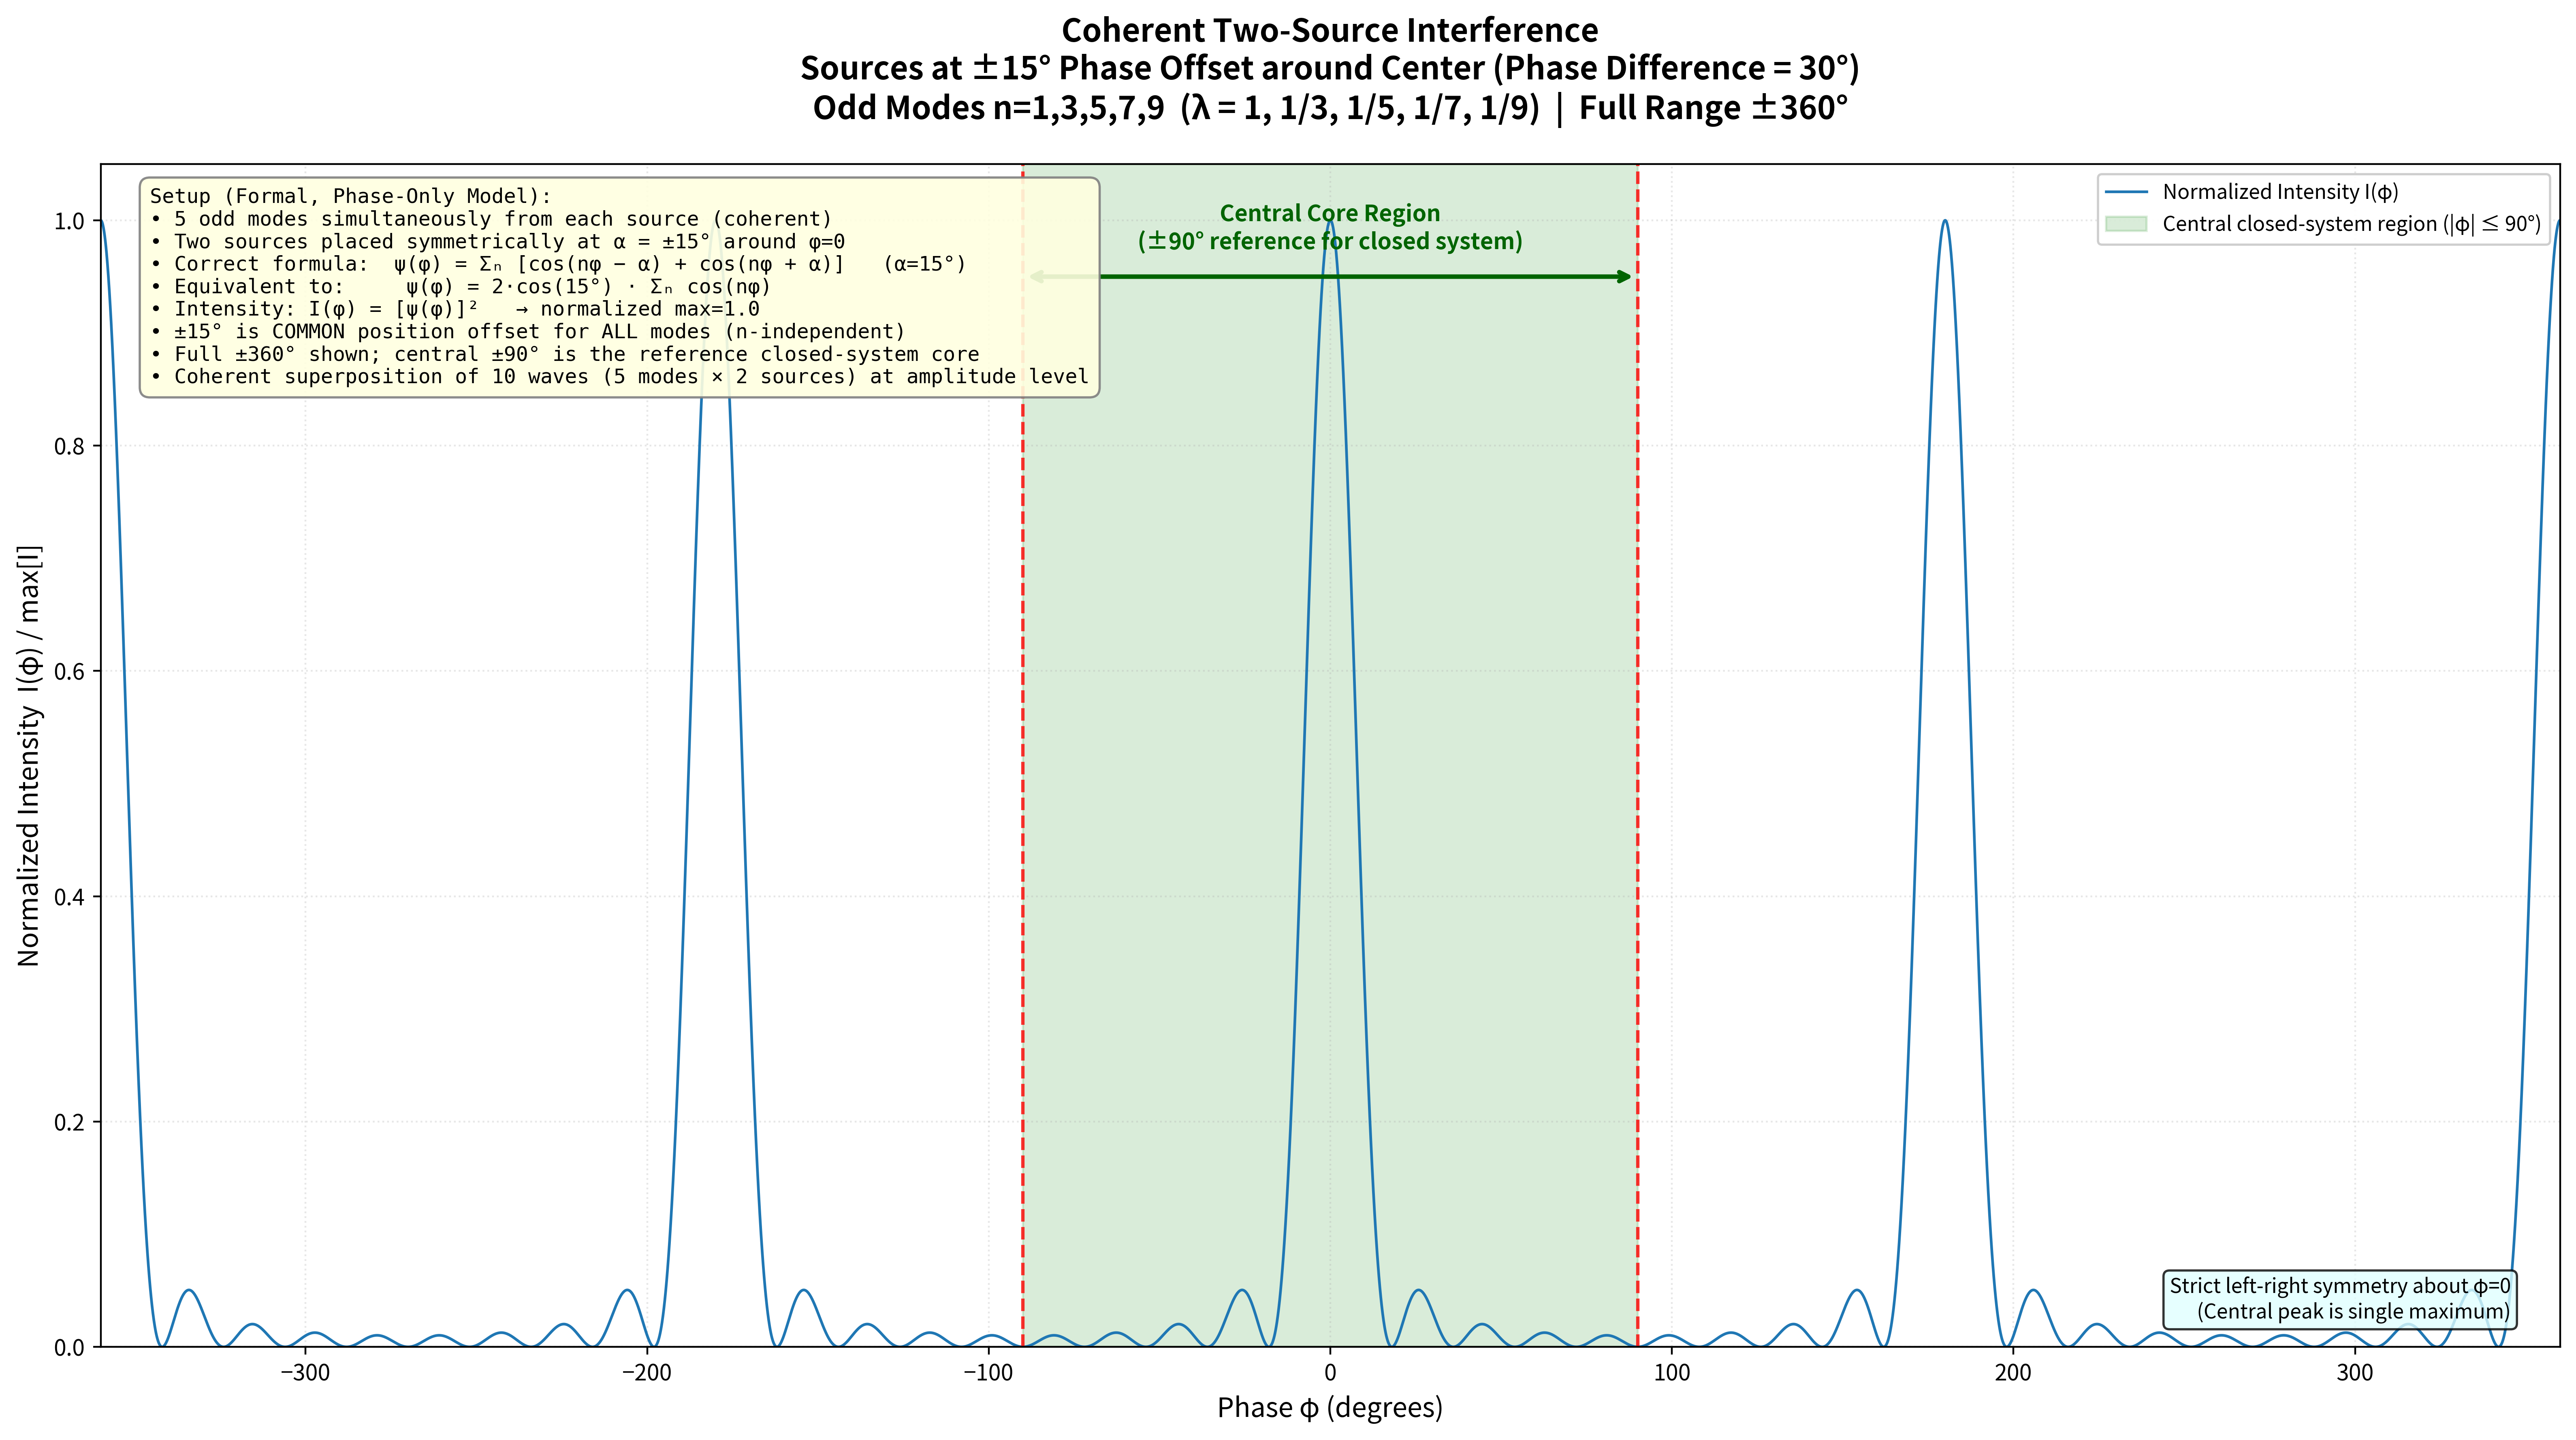
\includegraphics[keepaspectratio,alt={図2}]{two_source_coherent_interference_corrected_v4_hires.png}}
\caption{図2}
\end{figure}

\textbf{図2}: 二コピー重ね合わせ \(I_\alpha\)（\(N=9\)、相対位相
\(2\alpha=30^\circ\)、すなわち
\(\alpha=15^\circ\)）の規格化二乗振幅。全域 \(\pm 360^\circ\)、中央
\(\pm 90^\circ\ (=\pm\pi/2)\)
を強調。規格化波形は単一コピーのものと一致する（波形不変性）。

\begin{center}\rule{0.5\linewidth}{0.5pt}\end{center}

\subsection{4. 結論}\label{ux7d50ux8ad6}

半波長位相区間 \(\varphi\in[-\pi/2,\pi/2]\) 上の一定振幅奇数倍音和
\(S_N\) の二つのコピーに、全倍音へ共通の相対位相 \(\pm\alpha\)
を与えて重ね合わせた波
\(\psi_\alpha=\sum[\cos(n\varphi-\alpha)+\cos(n\varphi+\alpha)]\)
について、和積の三角恒等式から

\[
\psi_\alpha(\varphi)=2\cos\alpha\cdot S_N(\varphi),
\qquad
I_\alpha(\varphi)=4\cos^2\!\alpha\cdot I_N(\varphi)
\]

を得た。この厳密な恒等式から、次の各結果が従う。

\textbf{(1) 波形不変性}

\begin{itemize}
\tightlist
\item
  規格化波形 \(\widehat{I}_\alpha=\widehat{I}_N\) は相対位相 \(\alpha\)
  に依存しない。形状・両端の零・主ピーク近傍の局在幅は、相対位相を変えても不変である。
\end{itemize}

\textbf{(2) コントラスト則}

\begin{itemize}
\tightlist
\item
  相対位相 \(2\alpha\) は、波形を変えずに二乗振幅を \(\cos^2\!\alpha\)
  倍する（式 (3.6)）。\(\alpha=0\) で最大、\(\alpha=\pi/2\) で零となる。
\end{itemize}

以上はいずれも、和積の三角恒等式
\(\cos(n\varphi-\alpha)+\cos(n\varphi+\alpha)=2\cos(n\varphi)\cos\alpha\)
を一定振幅奇数倍音和に適用しただけの初等的な事実であり、物理的解釈は与えない。

\begin{center}\rule{0.5\linewidth}{0.5pt}\end{center}

\subsection{参考文献}\label{ux53c2ux8003ux6587ux732e}

{[}1{]}
高木貞治『解析概論』改訂第3版、岩波書店、1961年（フーリエ級数の章：三角級数、余弦和の閉じた形、和積の公式）。

\end{document}
